\documentclass[11pt]{beamer}
% \usetheme{Boadilla}
  \usetheme{default}


% acronyms for text or math mode
\newcommand {\ccast} {\mbox{\small CCAST}}
\newcommand {\cris} {\mbox{\small CrIS}}

\newcommand {\airs} {\mbox{\small AIRS}}
\newcommand {\iasi} {\mbox{\small IASI}}
\newcommand {\idps} {\mbox{\small IDPS}}
\newcommand {\nasa} {\mbox{\small NASA}}
\newcommand {\noaa} {\mbox{\small NOAA}}
\newcommand {\nstar} {\mbox{\small STAR}}
\newcommand {\umbc} {\mbox{\small UMBC}}
\newcommand {\uw}   {\mbox{\small UW}}

\newcommand {\fft}  {\mbox{\small FFT}}
\newcommand {\ifft} {\mbox{\small IFFT}}
\newcommand {\fir}  {\mbox{\small FIR}}
\newcommand {\fov}  {\mbox{\small FOV}}
\newcommand {\for}  {\mbox{\small FOR}}
\newcommand {\ict}  {\mbox{\small ICT}}
\newcommand {\ils}  {\mbox{\small ILS}}
\newcommand {\igm}  {\mbox{\small IGM}}
\newcommand {\opd}  {\mbox{\small OPD}}
\newcommand {\rms}  {\mbox{\small RMS}}
\newcommand {\zpd}  {\mbox{\small ZPD}}
\newcommand {\ppm}  {\mbox{\small PPM}}
\newcommand {\srf}  {\mbox{\small SRF}}
\newcommand {\sdr}  {\mbox{\small SDR}}

\newcommand {\ES} {\mbox{\small ES}}
\newcommand {\SP} {\mbox{\small SP}}
\newcommand {\IT} {\mbox{\small IT}}
\newcommand {\SA} {\mbox{\small SA}}

\newcommand {\ET} {\mbox{\small ET}}
\newcommand {\FT} {\mbox{\small FT}}

% abbreviations, mainly for math mode
\newcommand {\real} {\mbox{real}}
\newcommand {\imag} {\mbox{imag}}
\newcommand {\atan} {\mbox{atan}}
\newcommand {\obs}  {\mbox{obs}}
\newcommand {\calc} {\mbox{calc}}
\newcommand {\sinc} {\mbox{sinc}}
\newcommand {\psinc} {\mbox{psinc}}
\newcommand {\std} {\mbox{std}}

% symbols, for math mode only
\newcommand {\wnum} {\mbox{cm$^{-1}$}}
\newcommand {\lmax} {L_{\mbox{\tiny max}}}
\newcommand {\vmax} {V_{\mbox{\tiny max}}}

\newcommand {\tauobs} {\tau_{\mbox{\tiny obs}}}
\newcommand {\taucal} {\tau_{\mbox{\tiny calc}}}
\newcommand {\Vdc}  {V_{\mbox{\tiny DC}}}

\newcommand {\rIT} {r_{\mbox{\tiny\textsc{ict}}}}
\newcommand {\rES} {r_{\mbox{\tiny\textsc{es}}}}
\newcommand {\robs} {r_{\mbox{\tiny obs}}}

\newcommand {\rITobs} {r_{\mbox{\tiny\textsc{ict}}}^{\mbox{\tiny obs}}}
\newcommand {\rITcal} {r_{\mbox{\tiny\textsc{ict}}}^{\mbox{\tiny cal}}}

\newcommand {\ITmean} {\langle\mbox{\small IT}\rangle}
\newcommand {\SPmean} {\langle\mbox{\small SP}\rangle}


\title{cris extended resolution \\
       calibration algorithm comparisons \\
\vspace{4mm}
{****} DRAFT {****} \\
}
\author{H.~E.~Motteler, L.~L.~Strow}
\institute{
  UMBC Atmospheric Spectroscopy Lab \\
  Joint Center for Earth Systems Technology \\
}
\date{\today}
\begin{document}

%----------- slide --------------------------------------------------%
\begin{frame}[plain]
\titlepage
\end{frame}
%----------- slide --------------------------------------------------%
\begin{frame}
\frametitle{introduction}

\begin{itemize}

  \item we compare the {\umbc} implementations of our {\ccast}
    reference and the \noaa~4 calibration algorithms on extended
    resolution data

  \item this allows for identical \ils\ and processing details---the
    only difference in tests is the form of the calibration equation

  \item we show results for clear matchups, comparing the {\ccast}
    algorithm with flat reference truth and \noaa~4 with reference
    truth convolved with instrument responsivity

  \item the respective residuals are very similar

\end{itemize}

\end{frame}
%----------- slide --------------------------------------------------%
\begin{frame}
\frametitle{methods}

\begin{itemize}

  \item for tests with calculated radiance we start with 3782 clear
    matchups from ccast granule SDR\_d20160120\_t0304487 and
    calculate upwelling radiances with kcarta at a 0.0025 cm-1 grid

  \item for the ``flat'' tests the ccast processing filters are
    applied pointwise and the result is convolved to the {\cris}
    user grid

  \item for the ``resp'' tests instrument responsivity is applied
    pointwise to the kcarta radiances, these are convolved to the
    user grid, and then divided pointwise by inverse responsivity

% \item relative tests are with data averaged over the three day
%   test period, 18-20 Jan 2016
    
  \item all test are done with periodic sinc wrapping at the sensor
    grid, cosine apodization of the extended res points, the old a2
    weights, and double Fourier interpolation to the user grid

\end{itemize}

\end{frame}
%----------- slide --------------------------------------------------%
\begin{frame}
\frametitle{responsivity vs flat reference truth}
\begin{center}
  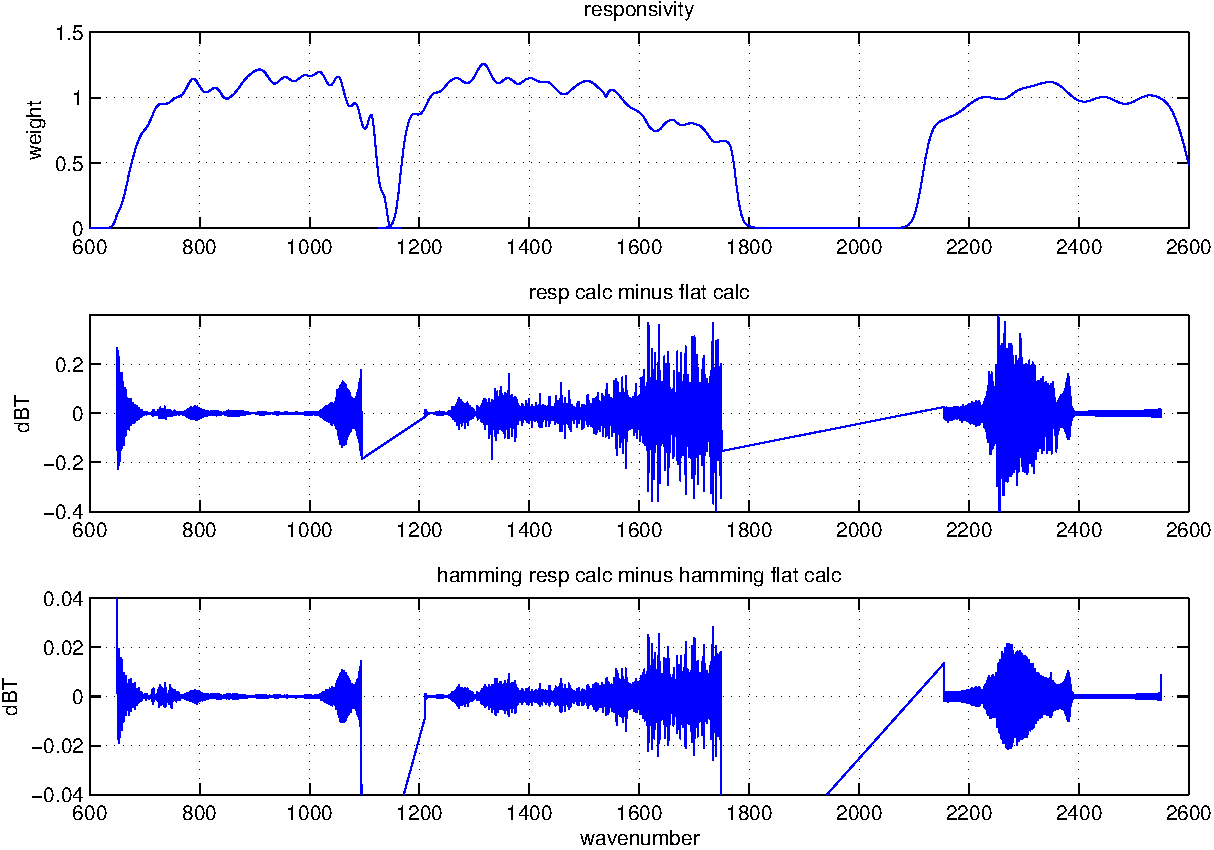
\includegraphics[scale=0.5]{figures/resp_flat_diff.pdf}
\end{center}
\end{frame}
%----------- slide --------------------------------------------------%
\begin{frame}
\frametitle{obs minus calc overview}
\begin{center}
  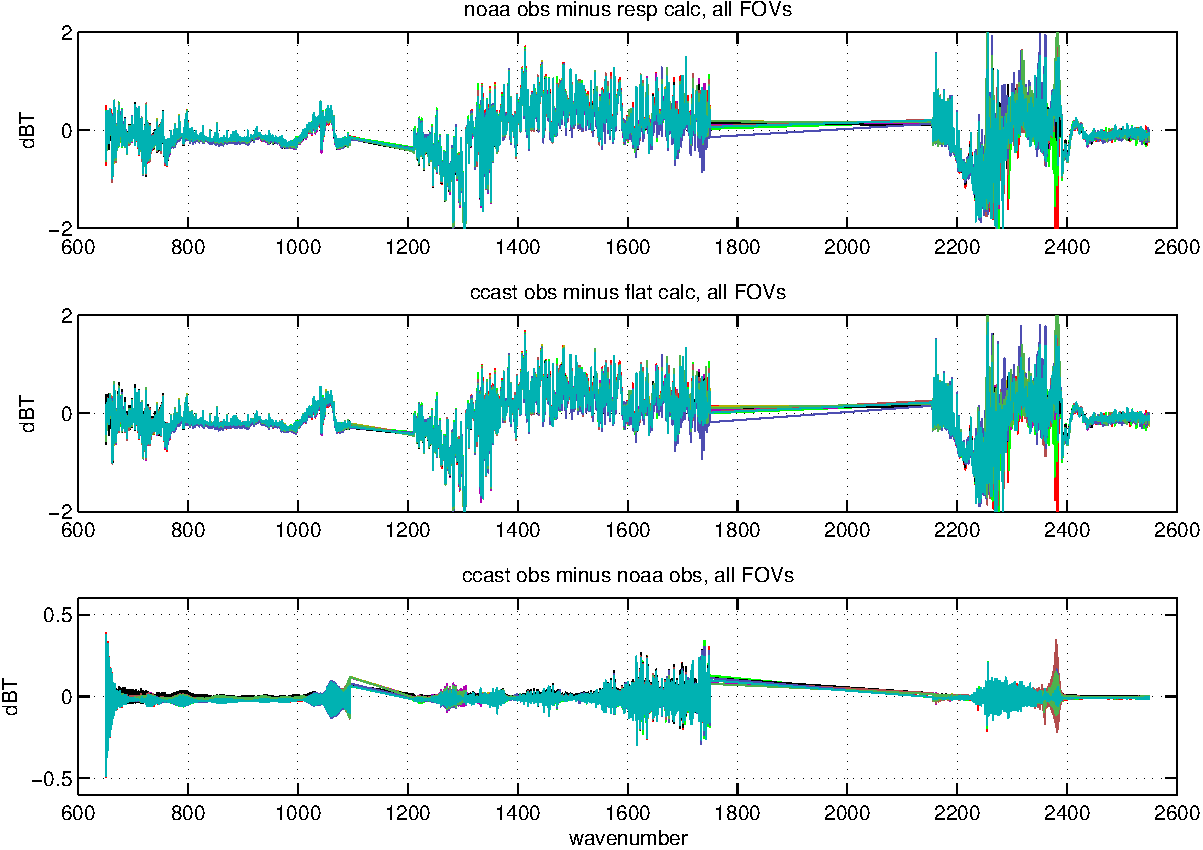
\includegraphics[scale=0.5]{figures/cal_summary.pdf}
\end{center}
\end{frame}
%----------- slide --------------------------------------------------%
\begin{frame}
\frametitle{obs and calc residuals}
\begin{center}
  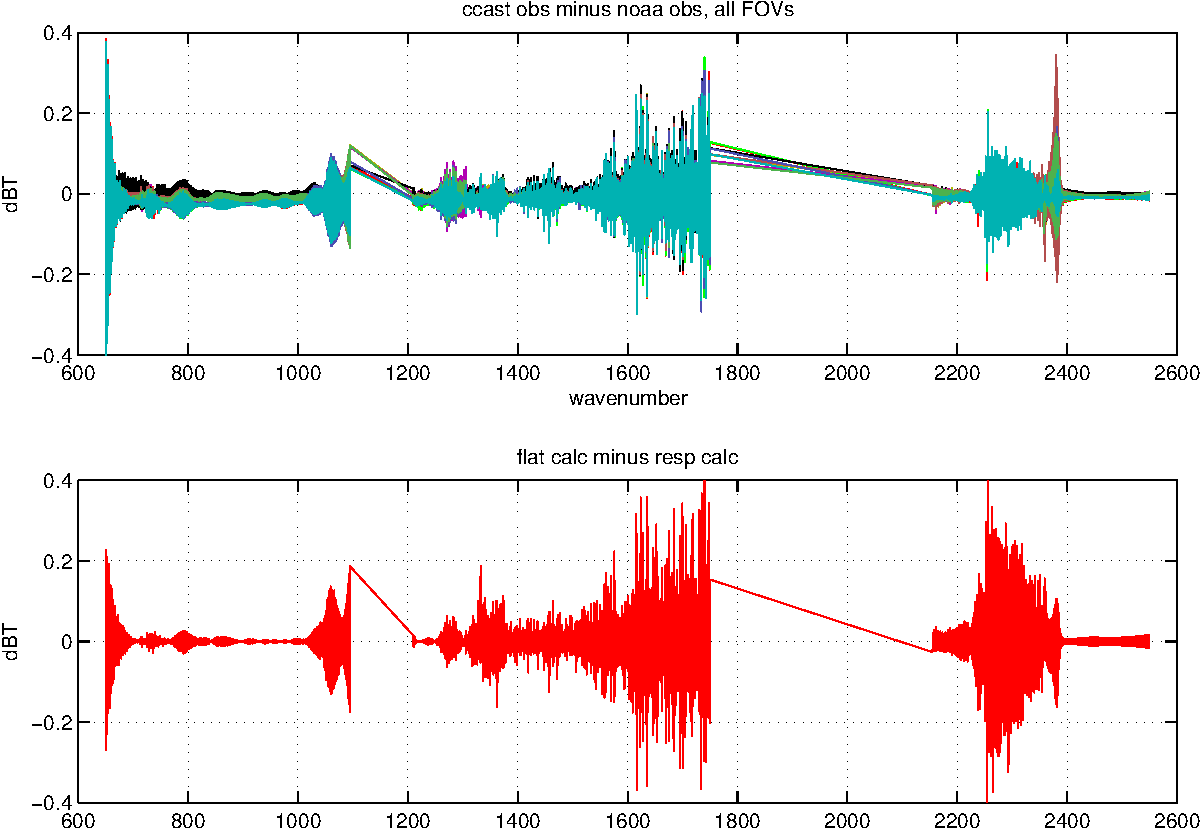
\includegraphics[scale=0.5]{figures/obs_calc_diffs.pdf}
\end{center}
\end{frame}
%----------- slide --------------------------------------------------%
\begin{frame}
\frametitle{obs minus calc LW detail}
\begin{center}
  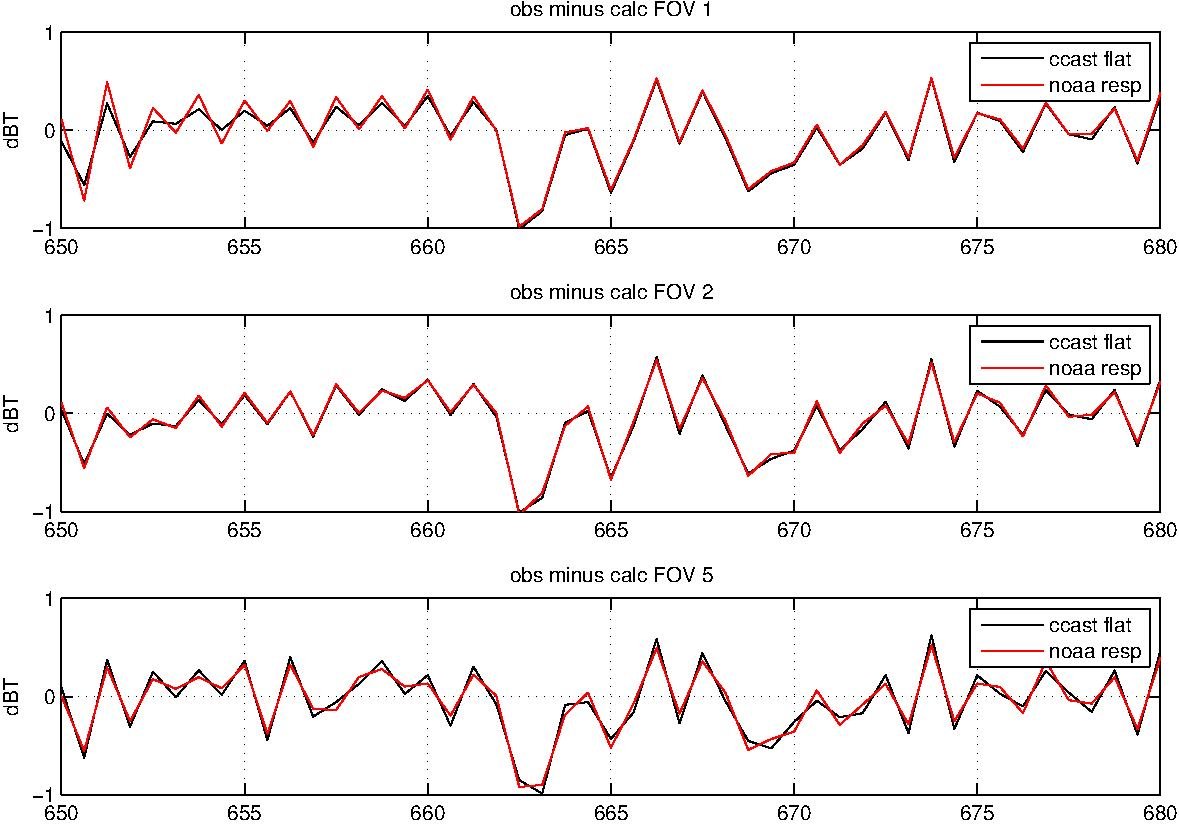
\includegraphics[scale=0.5]{figures/cal_LW_detail.pdf}
\end{center}
\end{frame}
%----------- slide --------------------------------------------------%
\begin{frame}
\frametitle{noaa all fovs LW detail}
\begin{center}
  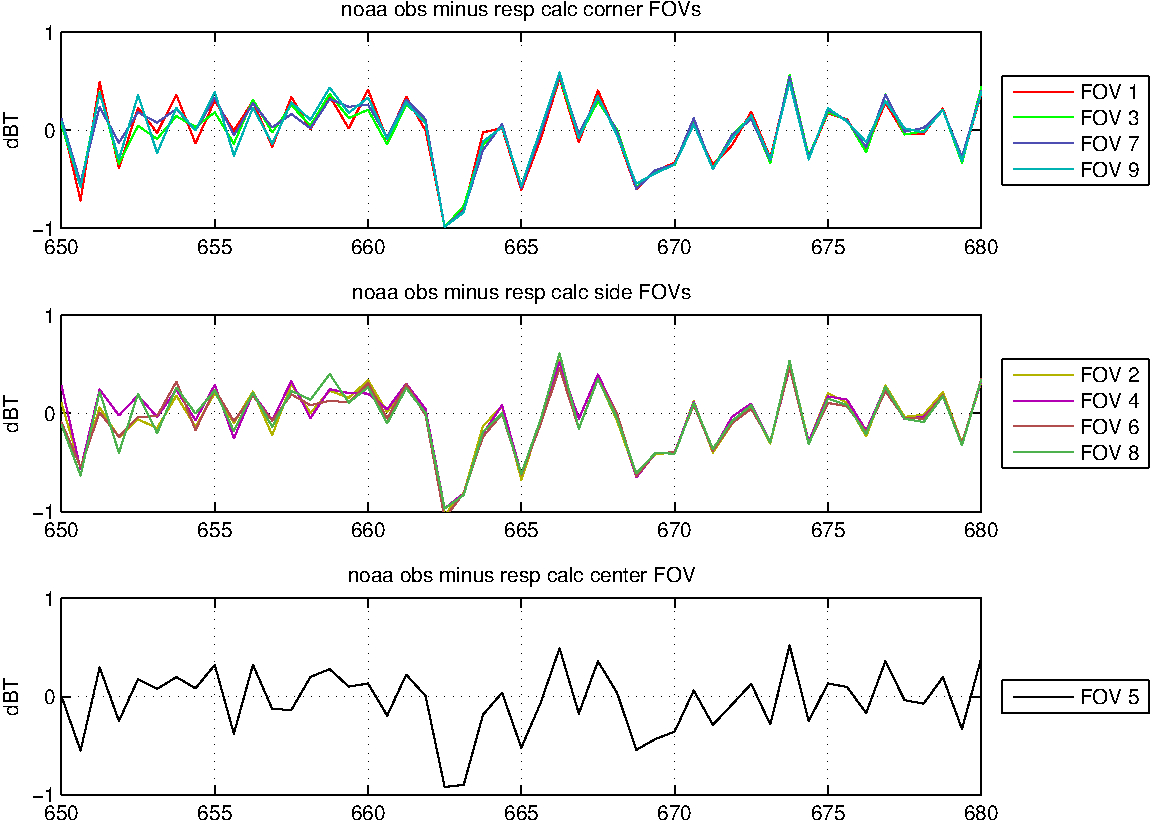
\includegraphics[scale=0.5]{figures/cal_noaa_LW.pdf}
\end{center}
\end{frame}
%----------- slide --------------------------------------------------%
\begin{frame}
\frametitle{ccast all fovs LW detail}
\begin{center}
  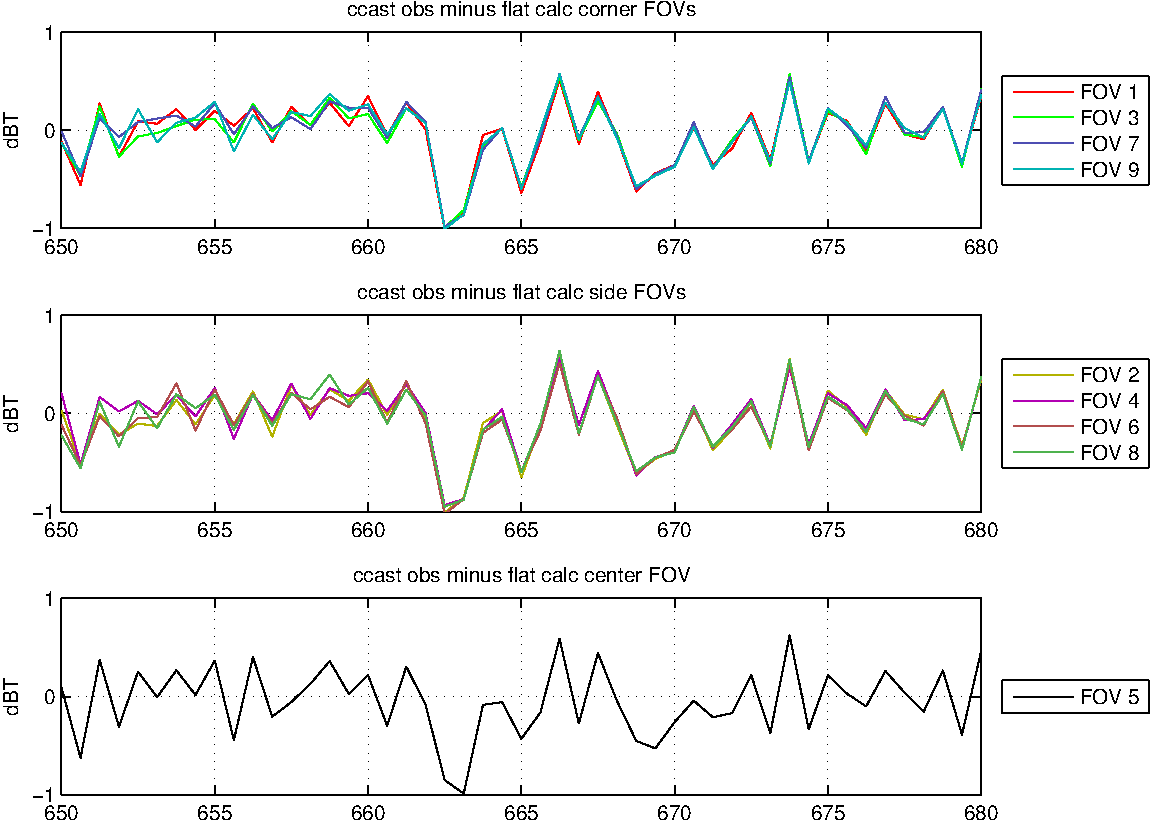
\includegraphics[scale=0.5]{figures/cal_ccast_LW.pdf}
\end{center}
\end{frame}
%----------- slide --------------------------------------------------%
\begin{frame}
\frametitle{obs minus calc MW detail}
\begin{center}
  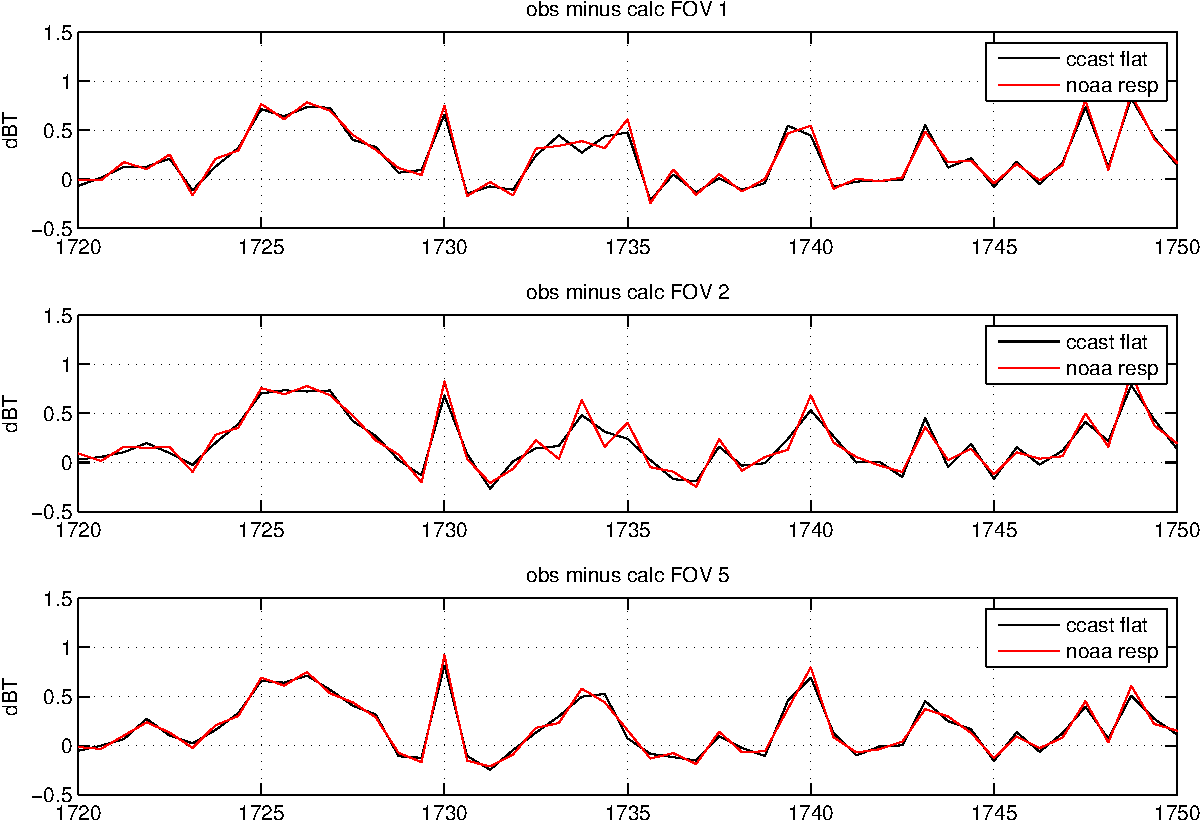
\includegraphics[scale=0.5]{figures/cal_MW_detail.pdf}
\end{center}
\end{frame}
%----------- slide --------------------------------------------------%
\begin{frame}
\frametitle{noaa all fovs MW detail}
\begin{center}
  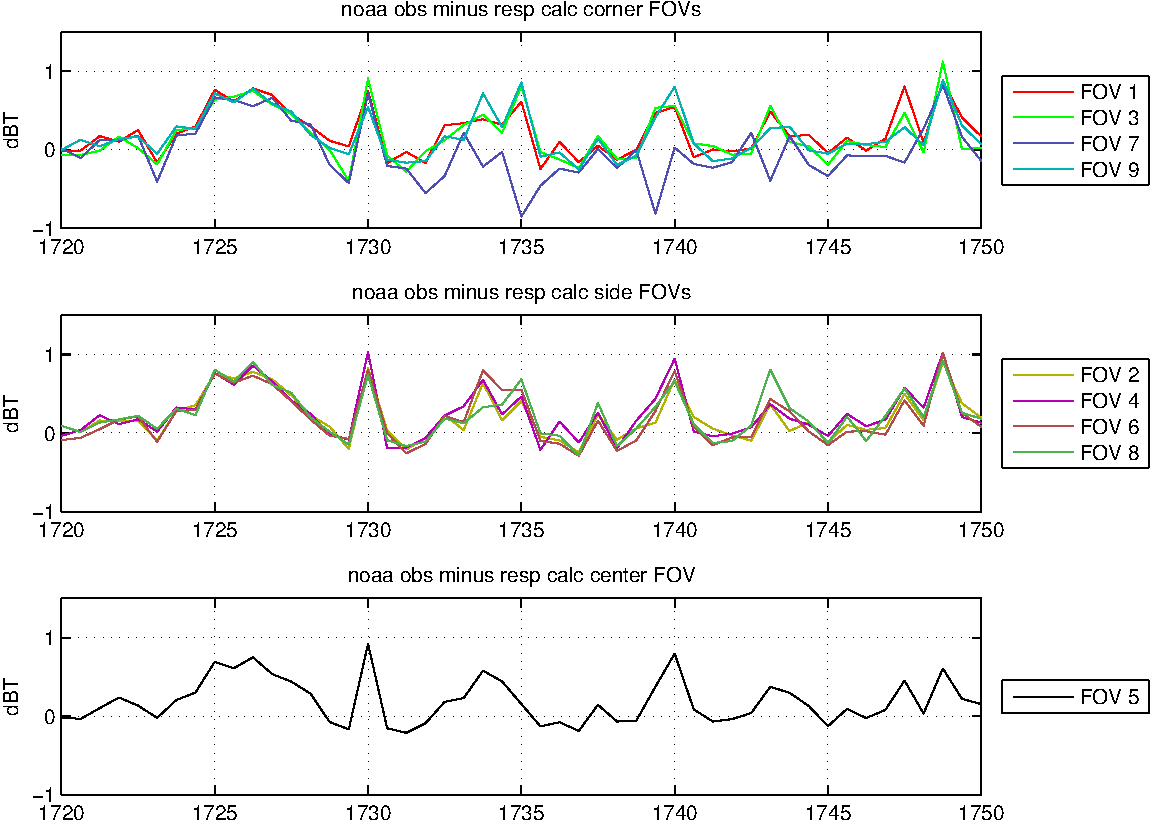
\includegraphics[scale=0.5]{figures/cal_noaa_MW.pdf}
\end{center}
\end{frame}
%----------- slide --------------------------------------------------%
\begin{frame}
\frametitle{ccast all fovs MW detail}
\begin{center}
  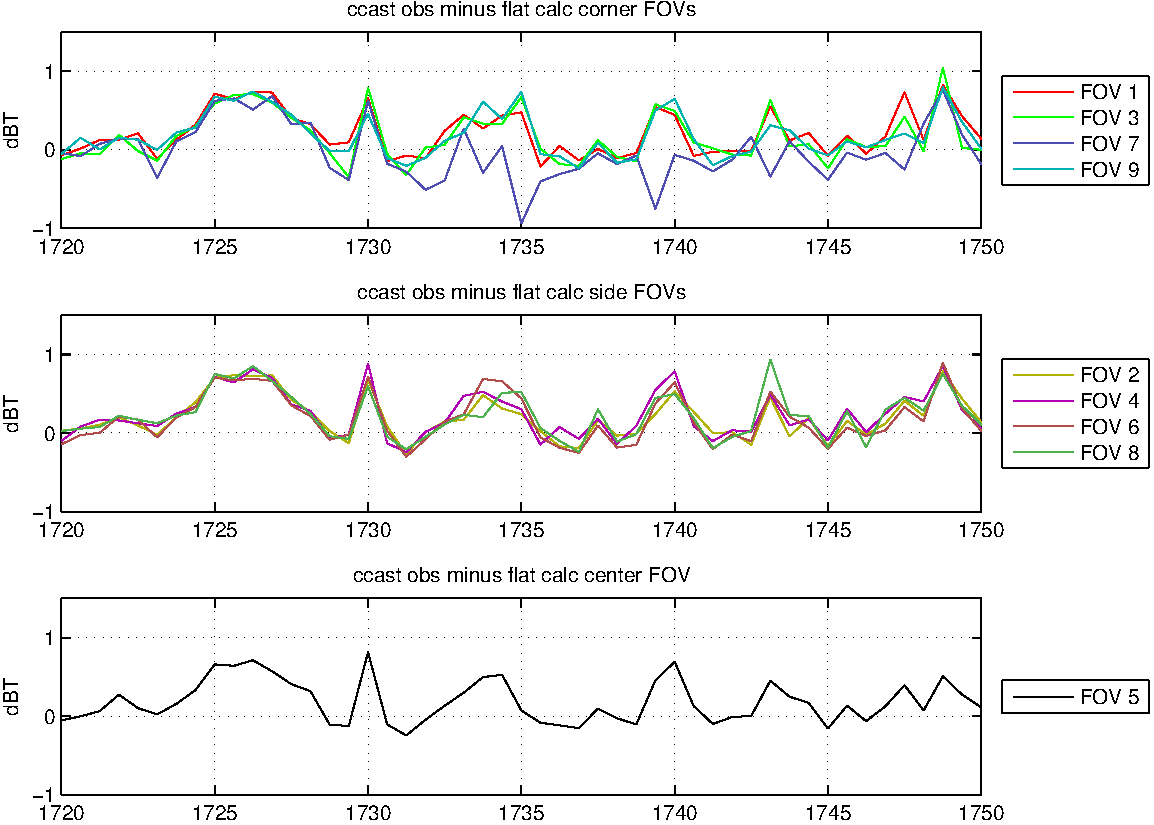
\includegraphics[scale=0.5]{figures/cal_ccast_MW.pdf}
\end{center}
\end{frame}
%----------- slide --------------------------------------------------%
\begin{frame}
\frametitle{obs minus calc SW detail}
\begin{center}
  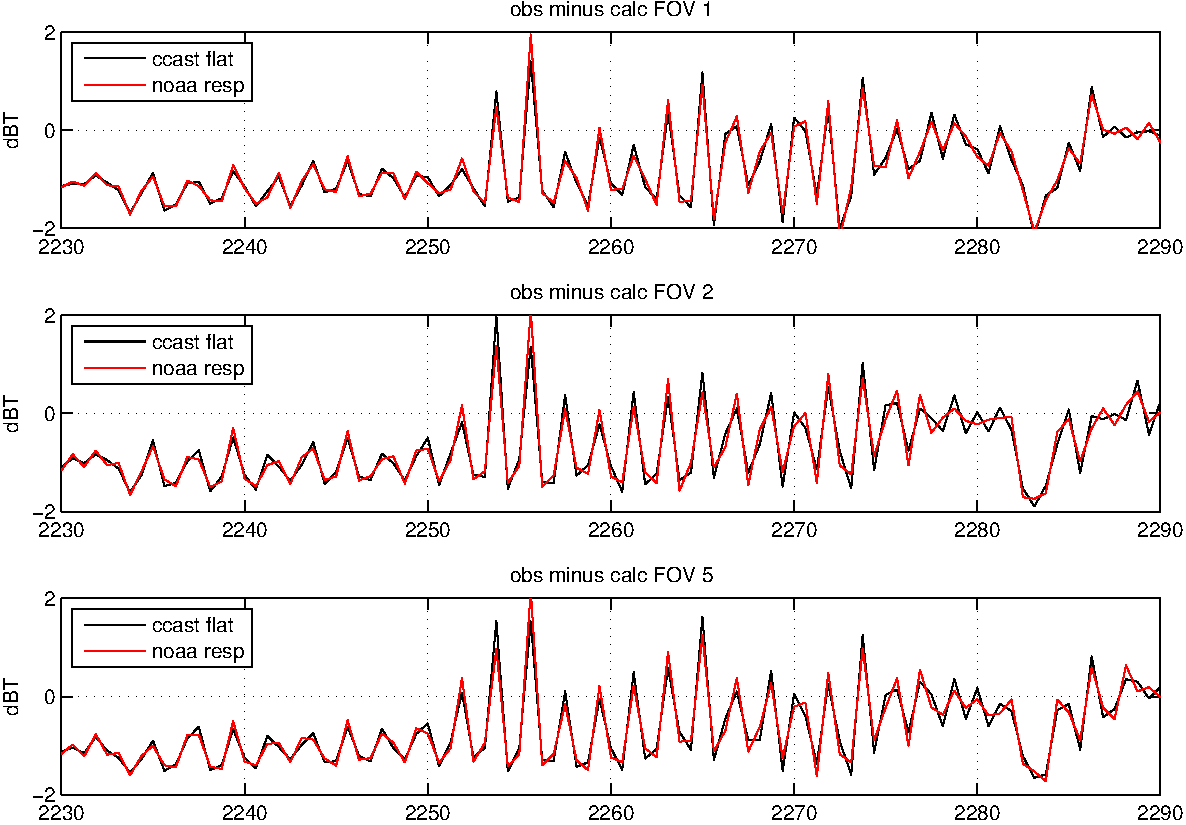
\includegraphics[scale=0.5]{figures/cal_SW_detail.pdf}
\end{center}
\end{frame}
%----------- slide --------------------------------------------------%
\begin{frame}
\frametitle{obs minus calc notes}

\begin{itemize}

  \item {\ccast} minus flat and {\noaa} minus resp residuals are
    similar, significantly more so than for earlier comparisons

  \item {\ccast} minus {\noaa} is similar to the responsivity
    residual

% \item the spectral intervals shown here here are regions where the
%   differences between the algorithms were greatest for our 15 Aug
%   2015 regular high resolution comparison

  \item below 680 \wn\ we see {\ccast} does slightly better for the
    side and corner FOVS, while {\noaa} is slightly better for FOV 5.  
    The {\ccast} residuals are more consistent across FOVs

  \item in the MW detail we see {\ccast} does slightly better for
    all FOVs.  These results are with the old a2 weights; the new
    UMBC a2 weights give a significant further reduction in the MW
    residuals

\end{itemize}

\end{frame}
%----------- slide --------------------------------------------------%
\begin{frame}
\frametitle{double differences}

\begin{itemize}

  \item the double difference subtracts a smoothed bias, leaving the
    high frequency components of the residual.

  \item noaa default test, with responsivity \\
    $(\mbox{\small noaa obs} - \mbox{\small resp calc}) - 
       (\mbox{\small hamming noaa obs} - 
        \mbox{\small hamming resp calc})$

  \item ccast default test, with flat passband \\
    $(\mbox{\small ccast obs} - \mbox{\small flat calc}) - 
       (\mbox{\small hamming ccast obs} - 
        \mbox{\small hamming flat calc})$

  \item noaa alternate test, with flat passband \\
    $(\mbox{\small noaa obs} - \mbox{\small flat calc}) - 
       (\mbox{\small hamming noaa obs} - 
        \mbox{\small hamming flat calc})$  

  \item ccast alternate test, with responsivity \\
    $(\mbox{\small ccast obs} - \mbox{\small resp calc}) - 
       (\mbox{\small hamming ccast obs} - 
        \mbox{\small hamming resp calc})$

\end{itemize}

\end{frame}
%----------- slide --------------------------------------------------%
\begin{frame}
\frametitle{noaa resp and ccast flat double diffs}
\begin{center}
  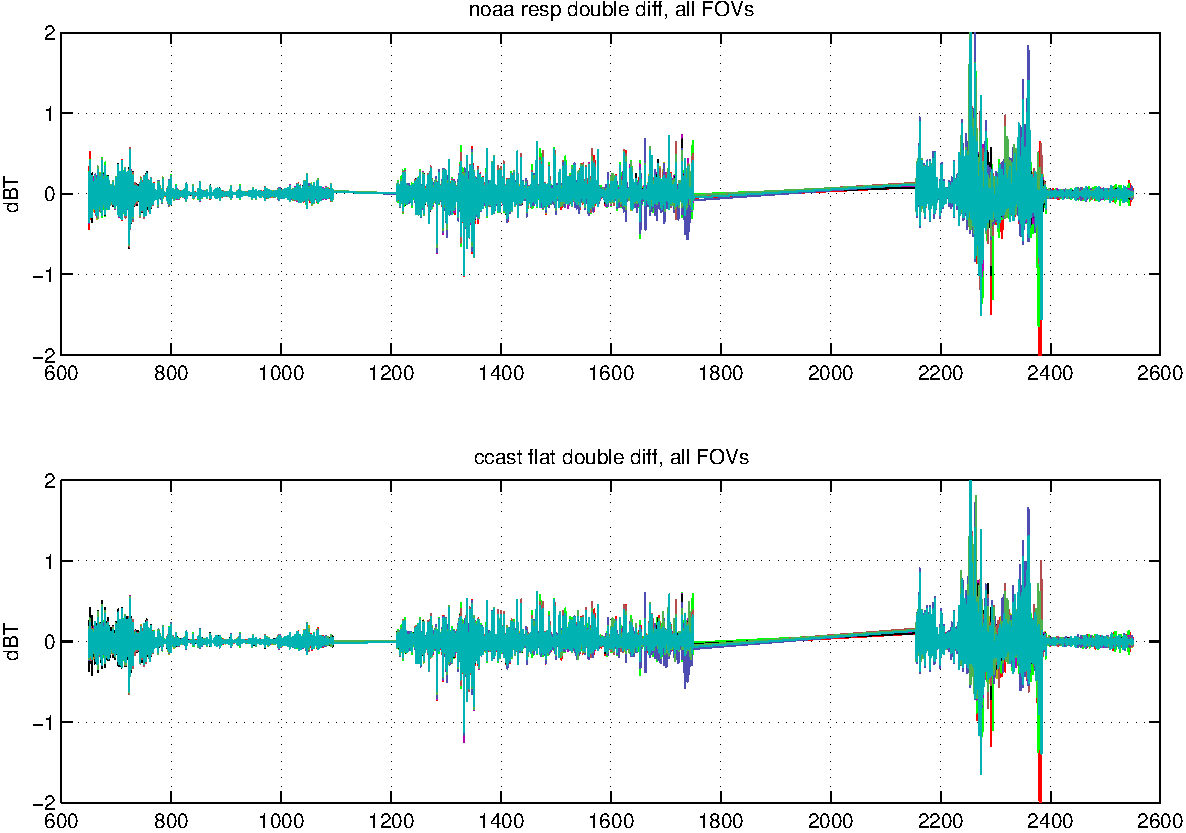
\includegraphics[scale=0.5]{figures/cal_ddif_1.pdf}
\end{center}
\end{frame}
%----------- slide --------------------------------------------------%
\begin{frame}
\frametitle{noaa flat and ccast resp double diffs}
\begin{center}
  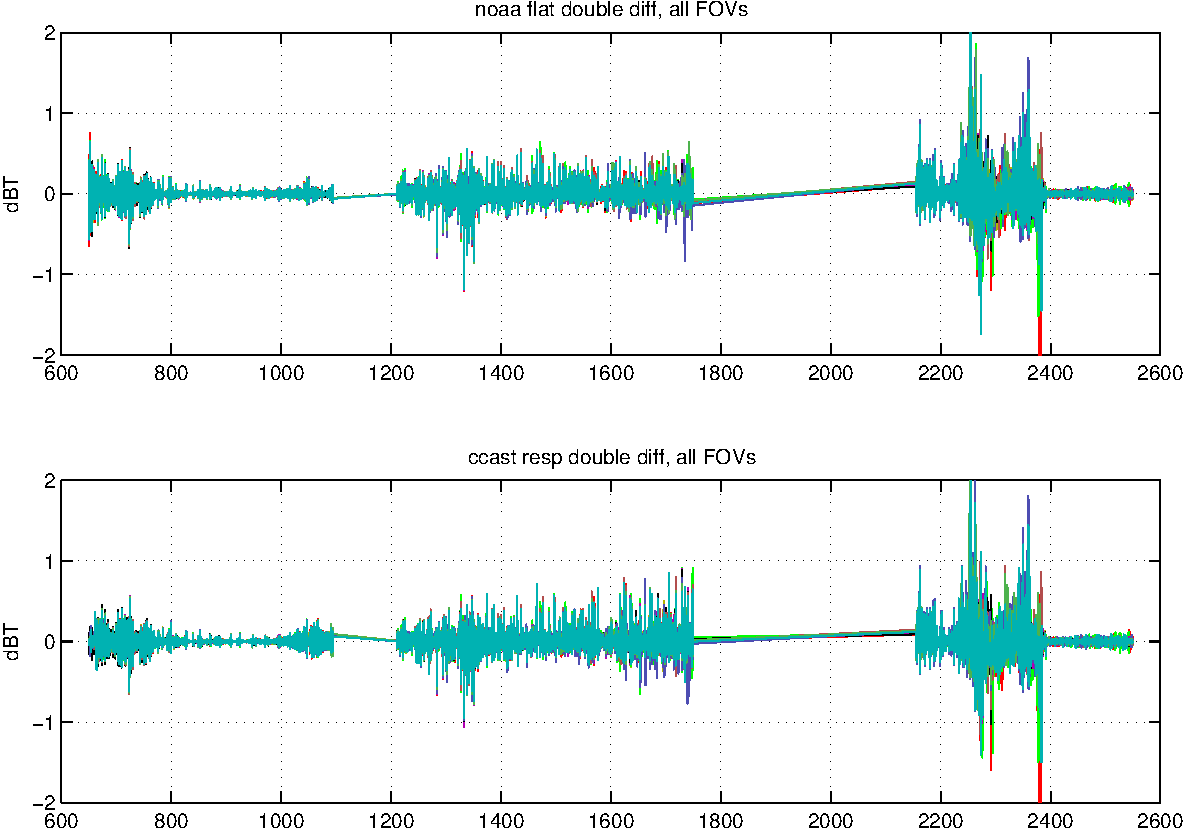
\includegraphics[scale=0.5]{figures/cal_ddif_2.pdf}
\end{center}
\end{frame}
%----------- slide --------------------------------------------------%
\begin{frame}
\frametitle{noaa resp and ccast flat LW band}
\begin{center}
  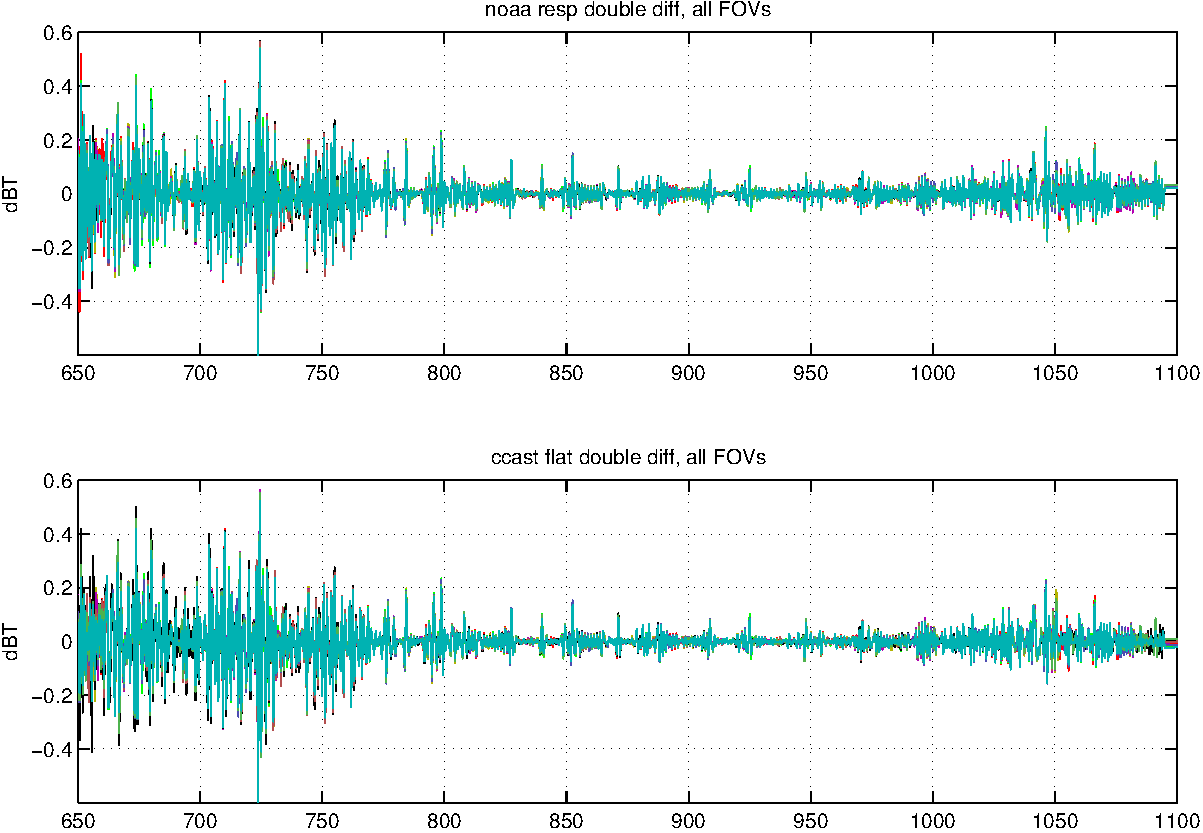
\includegraphics[scale=0.5]{figures/ddif_LW_band.pdf}
\end{center}
\end{frame}
%----------- slide --------------------------------------------------%
\begin{frame}
\frametitle{noaa resp and ccast flat LW zoom}
\begin{center}
  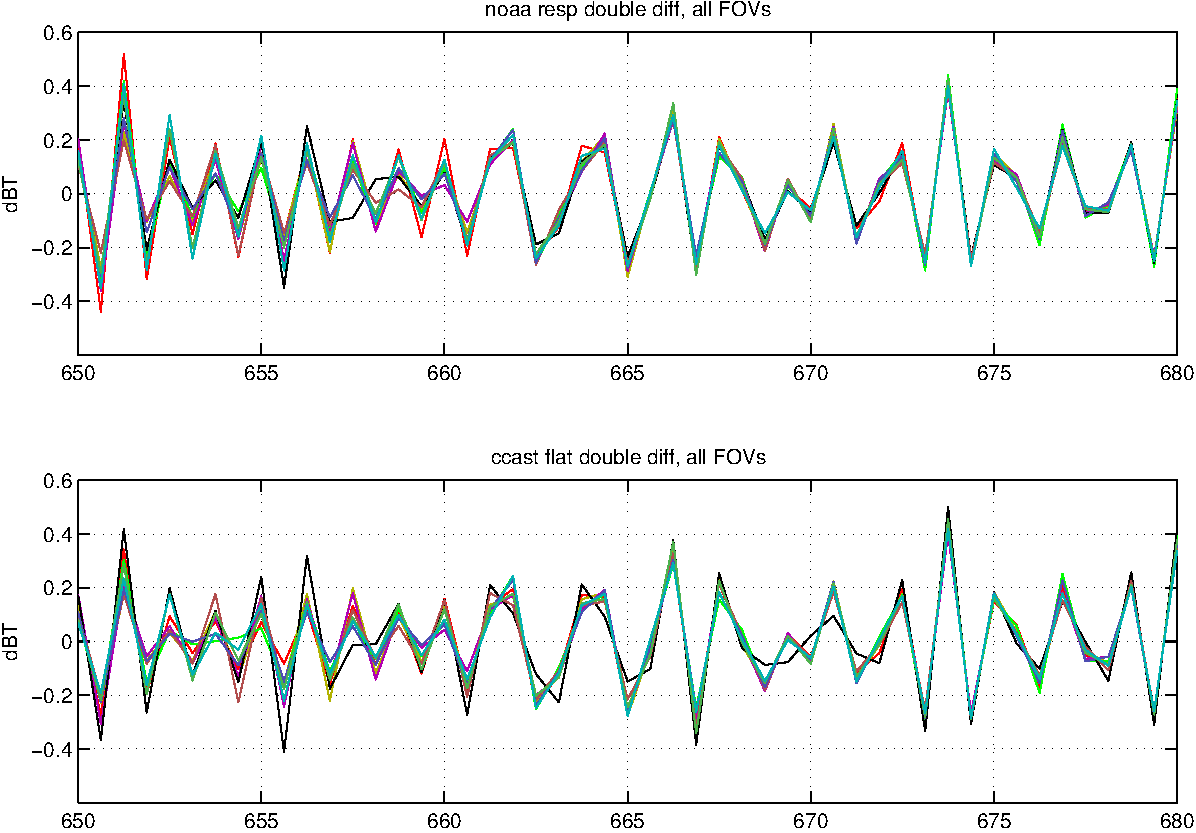
\includegraphics[scale=0.5]{figures/ddif_LW_zoom.pdf}
\end{center}
\end{frame}
%----------- slide --------------------------------------------------%
\begin{frame}
\frametitle{noaa resp and ccast flat MW band}
\begin{center}
  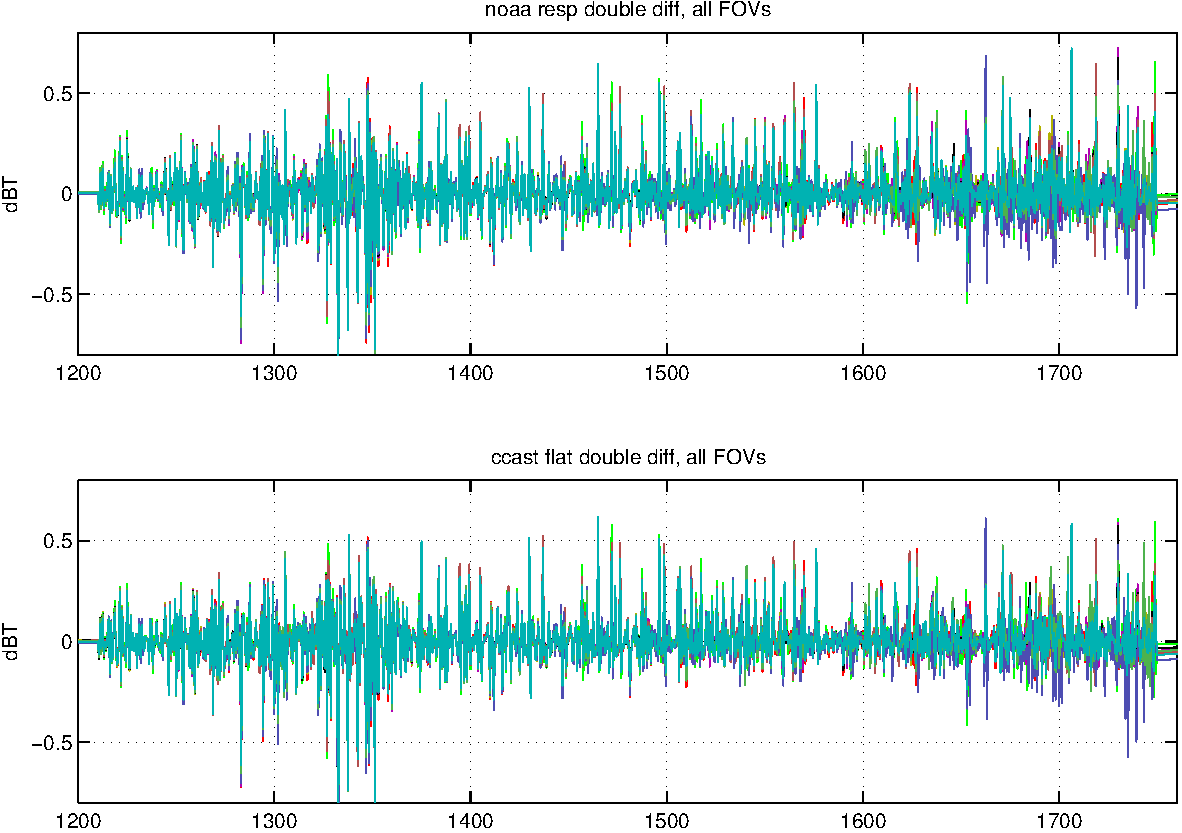
\includegraphics[scale=0.5]{figures/ddif_MW_band.pdf}
\end{center}
\end{frame}
%----------- slide --------------------------------------------------%
\begin{frame}
\frametitle{noaa resp and ccast flat MW zoom}
\begin{center}
  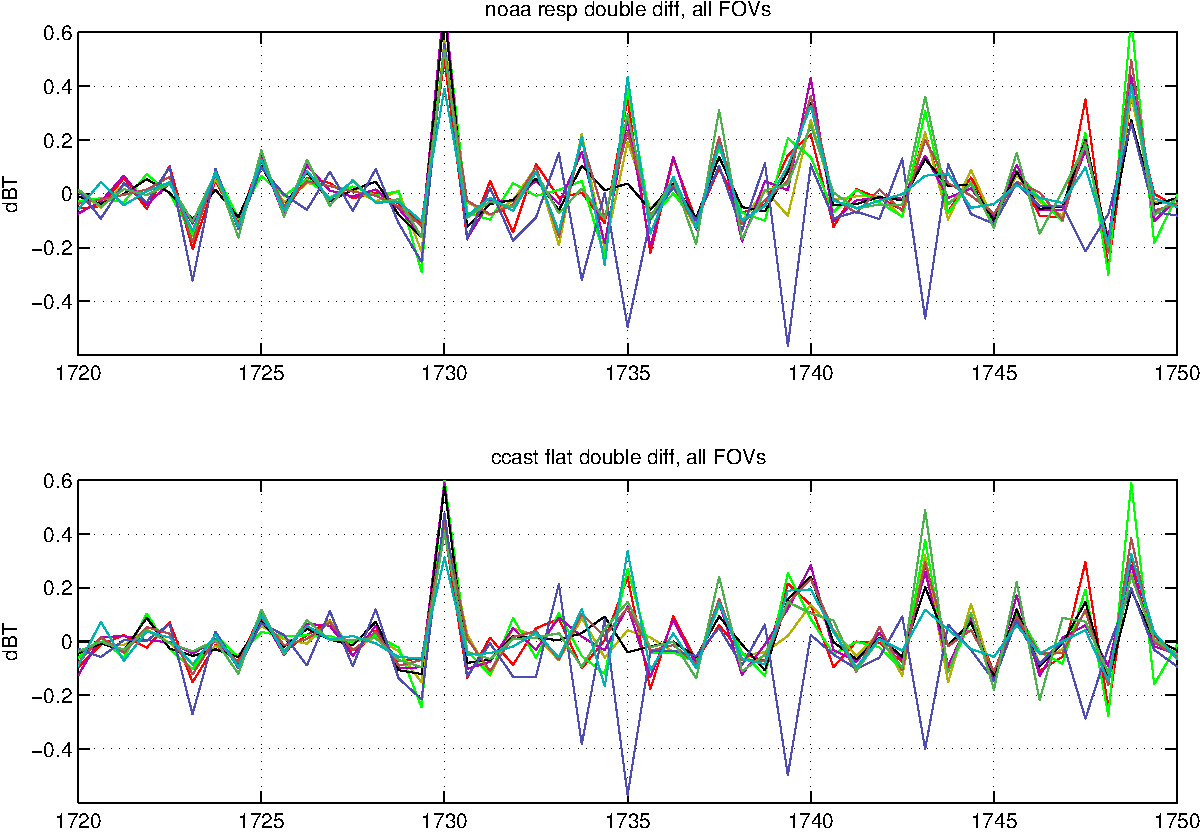
\includegraphics[scale=0.5]{figures/ddif_MW_zoom.pdf}
\end{center}
\end{frame}
%----------- slide --------------------------------------------------%
\begin{frame}
\frametitle{double difference notes}

\begin{itemize}

  \item double differences do not show a significant difference
    between the algorithms compared with their respective reference
    truths

% \item the {\ccast} minus flat and {\noaa} minus resp double
%   differences are very similar

  \item LW residuals are quite similar for both the full band and
    the selected zoom

  \item MW residuals are also quite similar, with {\ccast} maybe
    slightly better above around 1600 cm-1.  

  \item swapping reference truth---comparing {\noaa} with flat
    reference truth and {\ccast} with responsivity, we see both do
    slightly worse overall than when compared with their default
    reference truths

\end{itemize}

\end{frame}
%----------- slide --------------------------------------------------%
\begin{frame}
\frametitle{conclusions}

\begin{itemize}

  \item with the switch to extended res, we have seen a significant
    convergence in calibration algorithm performance 

%   when algorithms
%   are compared with their respective reference truths

  \item the {\noaa} ``SA-1 first'' algorithm does slightly better
    when compared with reference truth convolved with responsivity,
    while the {\ccast} ``ratio first'' algorithm does slightly
    better when compared with reference truth convolved with a flat
    passband

  \item this may be because responsivity cancels out more completely
    in the ratio-first method

  \item because reference truth convolved with a flat passband is
    a more conventional and non instrument-specific standard, the
    ccast algorithm (or perhaps some related ratio-first method) may
    be preferable

\end{itemize}

\end{frame}
%----------- slide --------------------------------------------------%
\end{document}

